% Phase 1 report. Each section lives in sections/<name>.tex and is written by its
% owner (see the section issues); this file only sets up the template and the order.
% Build from this folder: `tectonic main.tex`, or pdflatex + bibtex (e.g. Overleaf).

\documentclass[conference]{IEEEtran}

\usepackage{iftex}
\ifXeTeX
  % Tectonic and xelatex: Times-like text to match pdflatex's IEEEtran output.
  \usepackage{fontspec}
  \defaultfontfeatures{Extension=.otf, UprightFont=*-regular, BoldFont=*-bold,
    ItalicFont=*-italic, BoldItalicFont=*-bolditalic}
  \setmainfont{texgyretermes}
  \setsansfont{texgyreheros}
  \setmonofont{texgyrecursor}
\fi
\usepackage{cite}
\usepackage{amsmath,amssymb}
\usepackage{graphicx}
\usepackage{url}
\usepackage{tikz}
\usetikzlibrary{arrows.meta,positioning}

\begin{document}

\title{Remaining Useful Life Prediction for Turbofan Engines\\
from Engineered Degradation Features:\\
Phase 1 Machine-Learning Baselines on C-MAPSS}

\author{\IEEEauthorblockN{Gokul VKS, Milind Bansal, Isha Tomar, Yashi Agrawal and Mohammad Affan Anas}
\IEEEauthorblockA{Newton School of Technology, Rishihood University\\
Code and results: \url{https://github.com/vks-g/cmapss-rul-hybrid}}}

\maketitle

% Abstract and index terms (issue #7).

\begin{abstract}
Remaining useful life (RUL) prediction estimates how many operating cycles an
engine has left before it fails. This report presents Phase~1 of a project that
compares engineered degradation features with sequence models on the NASA C-MAPSS
turbofan data: feature-based machine-learning baselines on subset FD001, under a
protocol that Phase~2 will reuse. Training engines are split by engine, every
preprocessing step is refitted inside each training fold, the RUL target is
uncapped, and each of the 100 official test engines is scored once at its last
cycle. From regime-normalized sensor readings we build 155 causal predictors
(rolling means, slopes and changes since each engine's first cycle) and tune
Random Forest, XGBoost and Elastic Net regressors on them and on 25 raw inputs.
The engineered Random Forest reaches a test RMSE of 27.55 cycles and an MAE of
17.67 cycles, and all six models lie within five RMSE cycles of each other. The
engineered features roughly halve the tree models' error near failure (RMSE 7.52
and 5.62 against 13.50 and 14.32 with raw inputs) but overestimate young engines,
and a single engine contributes 92\% of the Random Forest's NASA score. Capping
the training target at 125 cycles lowers the Random Forest's RMSE to 16.21 with
engineered and 18.66 with raw inputs, reversing their order.
\end{abstract}

\begin{IEEEkeywords}
remaining useful life, predictive maintenance, C-MAPSS, feature engineering,
random forest, XGBoost, elastic net
\end{IEEEkeywords}


% Introduction (issue #7).

\section{Introduction}
\label{sec:introduction}

An aircraft engine that fails in service grounds the aircraft and can endanger it,
while an engine that is overhauled too early wastes useful life. Predictive
maintenance resolves this trade-off by estimating, from the engine's own sensor
history, its remaining useful life (RUL): the number of operating cycles left
before failure~\cite{Jardine2006review,Lei2018machinery}. Because run-to-failure
records of real engines are rare, most data-driven work uses NASA's C-MAPSS
simulation data~\cite{Saxena2008damage,Saxena2008turbofan}, in which every
training engine is observed until it fails and every test engine stops at an
unknown point before failure.

This project asks whether hand-engineered degradation features are enough for RUL
prediction, or whether models that learn directly from raw sensor sequences do
better. Fixed rolling summaries of recent history may miss long degradation
trajectories and interactions whose timing differs from engine to engine, which
sequence models are designed to capture~\cite{Zheng2017long}. Answering the
question fairly needs a strong feature-based baseline and an evaluation protocol
that both model families share. Published C-MAPSS results are hard to compare
because they differ in subsets, targets and protocols~\cite{Ramasso2014performance}.

Phase~1, reported here, builds that baseline on FD001, the subset with one
operating condition and one fault mode. Its contributions are:
\begin{itemize}
\item a leakage-controlled protocol, fixed for Phase~2: engine-grouped
  cross-validation, preprocessing refitted inside every training fold, an
  uncapped RUL target, and scoring of each official test engine once at its last
  cycle with RMSE, MAE and the asymmetric NASA score, overall and by degradation
  stage;
\item a causal feature set of 155 predictors per cycle (regime-normalized sensor
  readings with rolling means, slopes and changes from each engine's first
  cycle), compared with 25 raw inputs;
\item Random Forest, XGBoost and Elastic Net models tuned under this protocol and
  scored on the 100 official FD001 test engines;
\item an error analysis showing that the engineered features roughly halve the
  tree models' error near failure but overestimate young engines, that the NASA
  score is dominated by single engines, and that capping the target reverses the
  raw-versus-engineered comparison.
\end{itemize}

Section~\ref{sec:literature_review} reviews related work and
Section~\ref{sec:dataset_eda} the data. Section~\ref{sec:methodology} defines the
problem and the protocol, Sections~\ref{sec:feature_engineering}
and~\ref{sec:models} describe the features and models, and
Section~\ref{sec:results} reports the results. Section~\ref{sec:conclusion}
concludes and outlines Phase~2.

% Literature review (Phase 1). Citation keys resolve against reports/phase1/refs.bib.
% Includes the papers gathered in the section issues (#12, #16, #19).

\section{Literature Review}
\label{sec:literature_review}

\subsection{Prognostics and Remaining Useful Life}
Condition-based maintenance schedules maintenance from the measured condition of a
machine rather than from a fixed calendar, and prognostics, estimating how long a
component can keep operating, is its forward-looking half~\cite{Jardine2006review}.
The quantity to estimate is the remaining useful life (RUL): the number of operating
cycles left before failure. Reviews group RUL methods into physics-based models,
which need an explicit model of the failure mechanism; data-driven models, which learn
degradation from condition-monitoring data; and hybrids of the two~\cite{Lei2018machinery}.
Statistical data-driven approaches, from regression on degradation signals to
stochastic-process models, are surveyed by Si et al.~\cite{Si2011remaining}.
Lei et al.~\cite{Lei2018machinery} divide the data-driven pipeline into data
acquisition, health-indicator construction, health-stage division and RUL prediction.
The last two steps motivate our reporting of errors separately for the early, middle
and late stages of degradation.

\subsection{The C-MAPSS Benchmark}
Run-to-failure data from real engines is scarce, so simulation fills the gap.
Saxena et al.~\cite{Saxena2008damage} generated turbofan degradation data with the
C-MAPSS simulator. Each engine starts from a random, unknown level of initial wear; a
fault then reduces the flow and efficiency of engine modules at an exponential rate,
and the engine fails when a health index built from its operating margins reaches zero.
The resulting data set~\cite{Saxena2008turbofan} contains four subsets, FD001 to FD004,
that combine one or six operating conditions with one or two fault modes. For test
engines it gives only a truncated trajectory and the true RUL at its last cycle.
Saxena et al.~\cite{Saxena2008damage} also defined the asymmetric score used in the
PHM08 challenge, which penalizes late predictions more heavily than early ones because
an unexpected failure costs more than early maintenance; a broader set of prognostic
metrics is discussed in~\cite{Saxena2008metrics}. Six years later, Ramasso and
Saxena~\cite{Ramasso2014performance} reviewed more than seventy publications on these
data. They found that the absence of benchmark results, together with misunderstandings
about how the subsets relate, made reported results hard to compare, and they named
sensor noise, changing operating conditions and multiple fault modes as the main
difficulties of the benchmark.

\subsection{Feature-Based Machine Learning}
Early solutions to the PHM08 challenge already show the two directions the field has
followed. Wang et al.~\cite{Wang2008similarity} built a library of degradation patterns
from training engines and estimated a test engine's RUL from the lives of the most
similar patterns, while Heimes~\cite{Heimes2008recurrent} trained a recurrent neural
network and placed second in the competition. Later work mapped sensor values to RUL
directly. Khelif et al.~\cite{Khelif2017direct} used support vector regression with
wrapper-based sensor selection, removing the need to estimate degradation states or a
failure threshold, and Mathew et al.~\cite{Mathew2017prediction} compared a range of
classical regressors on the NASA turbofan data. Tree ensembles are also established
outside turbofans: for tool-wear prediction, Wu et al.~\cite{Wu2017comparative} found a
random forest more accurate than feed-forward networks and support vector regression.
On C-MAPSS, Wang et al.~\cite{Wang2023remaining} used random-forest importance to choose
the inputs of a neural regressor.

Our Phase~1 baselines follow this direct-regression line with three model families
chosen for complementary behavior. Random forests~\cite{Breiman2001random} average
many decorrelated regression trees, capturing non-linear sensor interactions with
little tuning. XGBoost~\cite{Chen2016xgboost} adds trees one at a time, each fitted to
the gradient of the loss of the current ensemble~\cite{Friedman2001greedy}, with
explicit regularization of tree complexity; it usually trades more tuning for higher
accuracy. The elastic
net~\cite{Zou2005regularization} is a linear model with combined $\ell_1$ and $\ell_2$
penalties whose grouping effect keeps strongly correlated predictors together, which
suits the redundant C-MAPSS sensors and gives an interpretable linear reference. All
three consume fixed-length summaries of each engine's recent history, such as rolling
means and slopes, rather than the raw sequence.

\subsection{Sequence Models and the Research Gap}
Deep learning removes the hand-crafted summary step. Convolutional networks applied to
fixed-length windows of raw sensor readings~\cite{SateeshBabu2016deep,Li2018remaining}
and long short-term memory (LSTM) networks~\cite{Hochreiter1997long,Zheng2017long} have
reported lower errors on C-MAPSS than the regression baselines they were compared with.
Zheng et al.~\cite{Zheng2017long} argue that features built from sliding windows do not
fully use the order of the sensor sequence. Many of these models are also trained
against a piecewise-linear target that is held constant early in life, when degradation
is not yet visible in the sensors, and decreases linearly
afterwards~\cite{Heimes2008recurrent,SateeshBabu2016deep,Zheng2017long,Li2018remaining}.

Two gaps motivate this project. First, fixed rolling features may miss long degradation
trajectories and interactions whose timing differs from engine to engine, which is what
sequence models are designed to capture. Second, as Ramasso and
Saxena~\cite{Ramasso2014performance} showed, published comparisons often differ in the
subsets, targets and evaluation protocols they use. Phase~1 therefore builds strong
feature-based baselines under a protocol that stays fixed for Phase~2: splits by engine
rather than by row, an uncapped RUL target with the capped target treated as an
ablation, and RMSE, MAE and the asymmetric score reported both overall and by
degradation stage.

\section{Dataset and Exploratory Analysis}
\label{sec:dataset_eda}

\subsection{The C-MAPSS Data Set}
We use the NASA C-MAPSS turbofan degradation data~\cite{Saxena2008turbofan},
generated with the simulator and damage-propagation model of Saxena
et al.~\cite{Saxena2008damage}. It has four subsets that differ in the number of
operating conditions and fault modes (Table~\ref{tab:subsets}). Every subset
has a training file, in which each engine is observed from an unknown initial
wear level until failure, and a test file, in which each trajectory stops at
some point before failure. A separate file gives the true RUL at the last
recorded cycle of each test engine. Engine identifiers are local to each
subset and split. FD001 is the primary subset of this project; the other three
show how the difficulty grows when operating conditions and fault modes are
mixed, which Ramasso and Saxena~\cite{Ramasso2014performance} identify as the
main obstacles to comparing results on this benchmark.

\begin{table}[!t]
\centering
\caption{C-MAPSS subsets. Engine and row counts are taken from the raw files;
lifetimes are the final cycles of the training engines.}
\label{tab:subsets}
\begin{tabular}{lcccccc}
\hline
Subset & Cond. & Faults & \multicolumn{2}{c}{Engines} & \multicolumn{2}{c}{Lifetime} \\
       &       &        & Train & Test & Median & Range \\
\hline
FD001 & 1 & 1 & 100 & 100 & 199   & 128--362 \\
FD002 & 6 & 1 & 260 & 259 & 199   & 128--378 \\
FD003 & 1 & 2 & 100 & 100 & 220.5 & 145--525 \\
FD004 & 6 & 2 & 249 & 248 & 234   & 128--543 \\
\hline
\end{tabular}
\end{table}

The fault mode is degradation of the high-pressure compressor (HPC) in FD001
and FD002; FD003 and FD004 add fan degradation. FD001 contains 20,631 training
rows and 13,096 test rows. Each row is one engine cycle with 26 columns: engine
identifier \texttt{unit}, cycle index \texttt{cycle}, three operating settings
\texttt{op\_1}--\texttt{op\_3} (altitude, Mach number and throttle resolver
angle) and 21 sensor channels $s_1,\dots,s_{21}$. The sensors record
temperatures, pressures, shaft speeds, ratios and bleed flows at different
engine stations; for example $s_2$, $s_3$ and $s_4$ are commonly identified
with the LPC, HPC and LPT outlet temperatures and $s_{11}$ with the HPC outlet
static pressure~\cite{Saxena2008damage}. RUL is not one of the columns. The
training target is the engine's final cycle minus the current cycle, and test
engines are scored only at their last observed cycle against the supplied RUL.

\subsection{Exploratory Findings}
The analysis below uses training trajectories only, so that no test
information shapes later modelling choices. It describes the data; the
transforms it motivates are fitted inside each training fold, as described in
Section~\ref{sec:feature_engineering}.

\subsubsection{Lifetimes differ widely between engines}
Fig.~\ref{fig:eda_lifetimes} shows that FD001 lifetimes range from 128 to 362
cycles around a median of 199, and the two-fault subsets are longer and more
spread out, reaching 525 and 543 cycles. Because an engine's rows are strongly
related to each other, a row-level split would place cycles of the same engine
on both sides of the split. All evaluation is therefore split by engine. The
long right tails also mean that the uncapped RUL target spans a wide range,
which inflates absolute errors on early-life cycles.

\begin{figure}[!t]
\centering
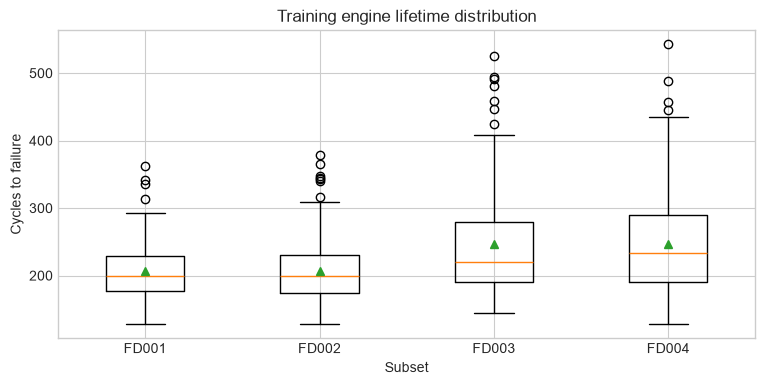
\includegraphics[width=\columnwidth]{../../results/figures/eda_lifetimes.png}
\caption{Distribution of training-engine lifetimes per subset. Triangles mark
the mean.}
\label{fig:eda_lifetimes}
\end{figure}

\subsubsection{Some sensors carry no information in FD001}
Six FD001 sensors are exactly constant across all training rows: $s_1$, $s_5$,
$s_{10}$, $s_{16}$, $s_{18}$ and $s_{19}$. They cannot separate healthy from
degraded engines, so the default selection rule removes them. Three further
channels, $s_6$, $s_8$ and $s_{13}$, vary very little relative to their mean,
but small variation is not the same as no information, and they are retained.
FD003 has five constant sensors, and FD002 and FD004 have none, because a
sensor that is fixed within one operating condition still changes between
conditions.

\subsubsection{Operating conditions dominate raw sensor levels}
The operating settings of FD002 and FD004 fall into six tight clusters
(Fig.~\ref{fig:eda_opsettings}), matching the six simulated flight conditions.
Fig.~\ref{fig:eda_hist} shows the consequence. In FD001 each sensor has a
single, roughly bell-shaped distribution, whereas in FD002 the same sensors
split into separate modes, one or more per condition, spread over a range much
wider than the change caused by degradation. Pooled statistics such as
correlations are therefore confounded by the operating condition in these
subsets. This finding motivates normalizing each sensor within its learned
operating regime before computing degradation features.

\begin{figure}[!t]
\centering
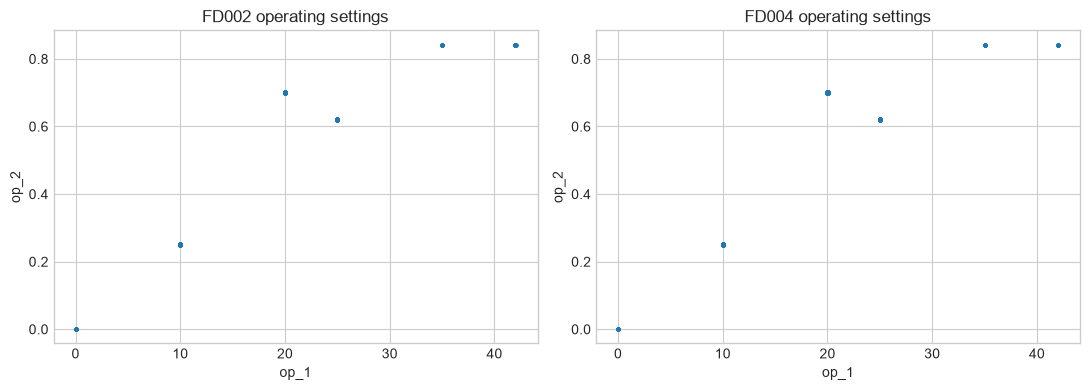
\includegraphics[width=\columnwidth]{../../results/figures/eda_op_settings.png}
\caption{Operating settings \texttt{op\_1} and \texttt{op\_2} for FD002 and FD004
training rows (10,000-row random samples). Each cluster is one operating
condition.}
\label{fig:eda_opsettings}
\end{figure}

\begin{figure*}[!t]
\centering
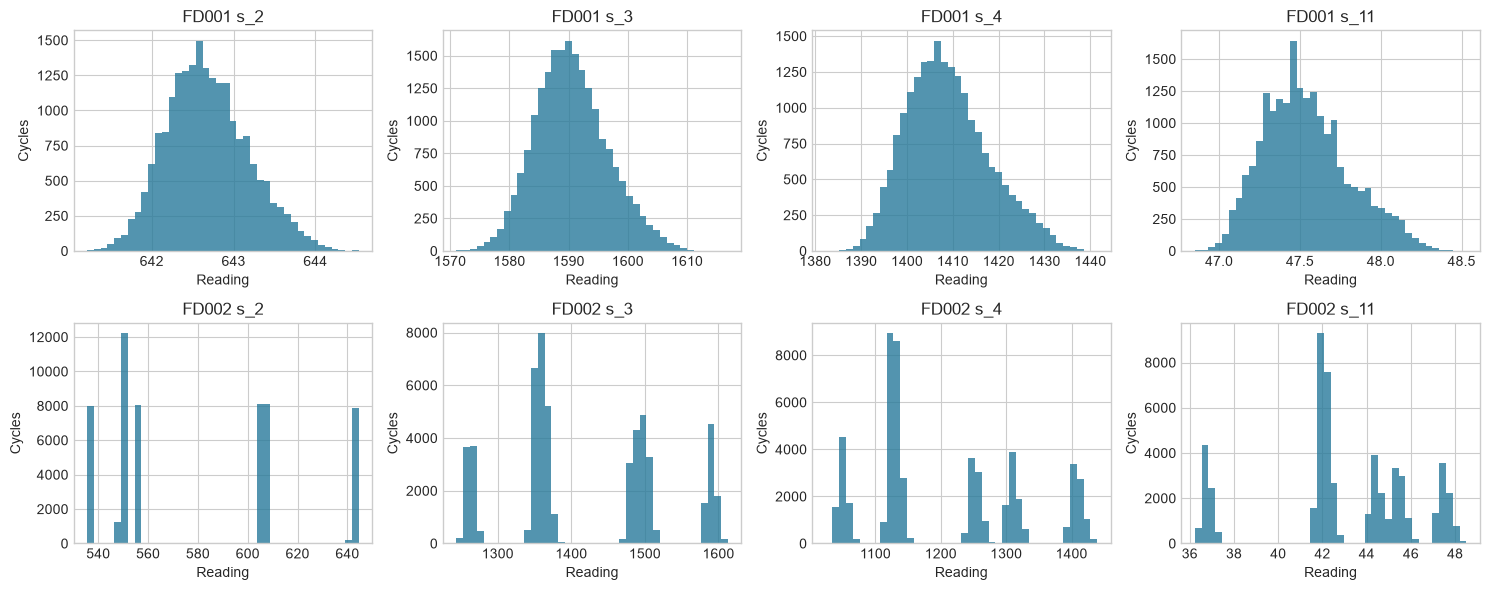
\includegraphics[width=\textwidth]{../../results/figures/eda_sensor_hist.png}
\caption{Raw readings of four sensors over all training cycles in FD001 (top,
one operating condition) and FD002 (bottom, six operating conditions).}
\label{fig:eda_hist}
\end{figure*}

\subsubsection{Degradation is slow early and accelerates near failure}
To compare engines of different lengths, Fig.~\ref{fig:eda_trends} averages
FD001 sensor readings in bins of the fraction of each engine's observed life.
The informative sensors $s_2$, $s_3$, $s_4$ and $s_{11}$ change little during
roughly the first half of life and then rise increasingly steeply until failure.
This shape is consistent with the exponential fault growth of the simulation
model~\cite{Saxena2008damage}. It has two implications. First, the level and
the recent slope of a sensor both carry information, which motivates the
rolling mean and slope features. Second, early-life cycles look alike in the
sensors while their true RUL differs widely, so errors on early cycles are
expected to be large under the uncapped target; this is why errors are broken
down by degradation stage and a capped target is checked as an ablation
(Section~\ref{sec:results}). The
life fraction uses each training engine's final cycle and is used here only
for description; it is never a model input. Individual engines are noisier
than these averages, and they start from different levels because initial
wear differs.

\begin{figure*}[!t]
\centering
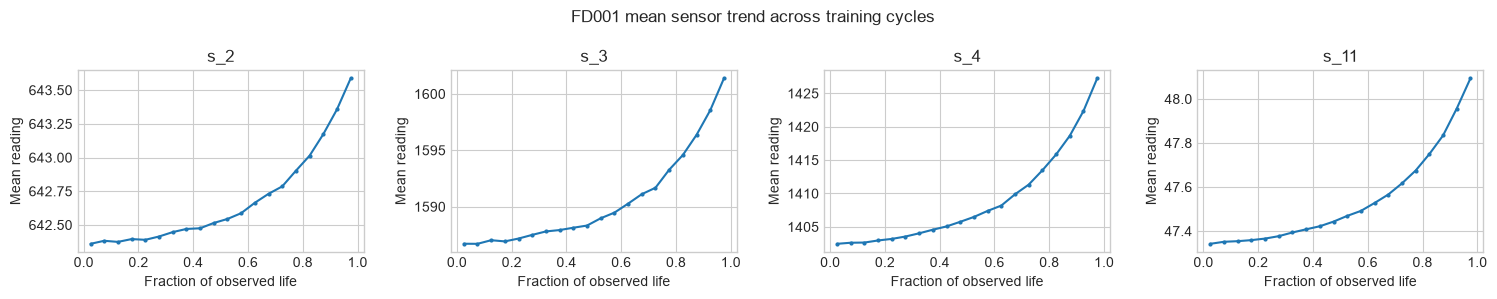
\includegraphics[width=\textwidth]{../../results/figures/eda_fd001_sensor_trends.png}
\caption{Mean FD001 training reading of four sensors in 20 bins of the fraction
of each engine's observed life.}
\label{fig:eda_trends}
\end{figure*}

% Methodology: problem definition and the evaluation protocol (issue #7).
% Features are in feature_engineering.tex and models in models.tex.

\section{Methodology}
\label{sec:methodology}

This section defines the prediction task and the evaluation protocol shared by
every Phase~1 model; Phase~2 keeps it unchanged. Fig.~\ref{fig:protocol}
summarizes the protocol. The features and models it evaluates are described in
Sections~\ref{sec:feature_engineering} and~\ref{sec:models}.

\begin{figure}[!t]
\centering
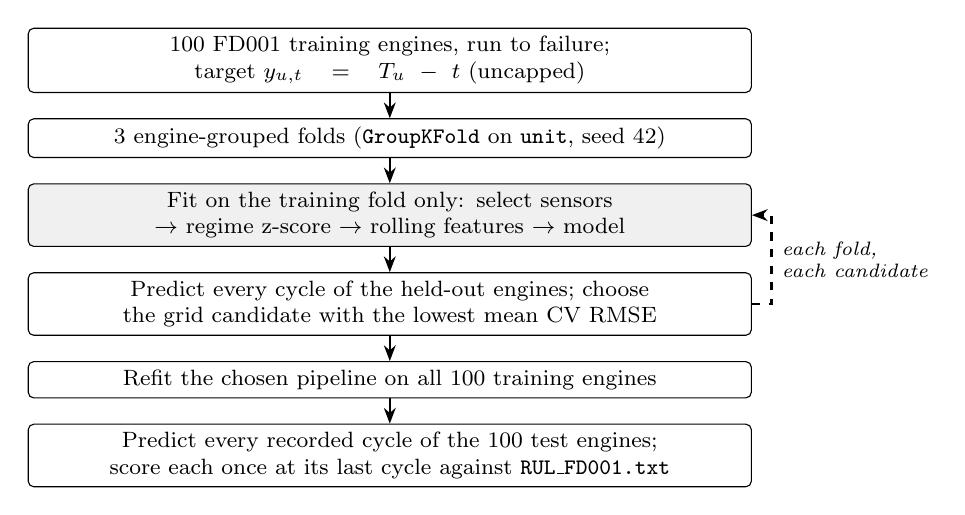
\begin{tikzpicture}[
    node distance=3.2mm,
    box/.style={draw, rounded corners=2pt, align=center, font=\footnotesize,
                 text width=0.74\columnwidth, inner sep=3pt},
    arrow/.style={-{Stealth[length=2mm]}, thick},
    note/.style={font=\scriptsize\itshape, align=left}]
  \node[box] (train) {100 FD001 training engines, run to failure;\\
    target $y_{u,t}=T_u-t$ (uncapped)};
  \node[box, below=of train] (folds) {3 engine-grouped folds
    (\texttt{GroupKFold} on \texttt{unit}, seed 42)};
  \node[box, below=of folds, fill=black!6] (fit) {Fit on the training fold only:
    select sensors $\rightarrow$ regime z-score $\rightarrow$ rolling features
    $\rightarrow$ model};
  \node[box, below=of fit] (cv) {Predict every cycle of the held-out engines;
    choose the grid candidate with the lowest mean CV RMSE};
  \node[box, below=of cv] (refit) {Refit the chosen pipeline on all 100 training
    engines};
  \node[box, below=of refit] (test) {Predict every recorded cycle of the 100 test
    engines; score each once at its last cycle against \texttt{RUL\_FD001.txt}};
  \draw[arrow] (train) -- (folds);
  \draw[arrow] (folds) -- (fit);
  \draw[arrow] (fit) -- (cv);
  \draw[arrow] (cv) -- (refit);
  \draw[arrow] (refit) -- (test);
  \draw[arrow, dashed] (cv.east) -- ++(2.5mm,0) |- (fit.east)
    node[note, pos=0.25, right] {each fold,\\each candidate};
\end{tikzpicture}
\caption{Evaluation protocol. Every data-dependent preprocessing step is part of
the pipeline (shaded), so it is refitted with the model inside each training
fold.}
\label{fig:protocol}
\end{figure}

\subsection{Problem Formulation}
Engine $u$ is observed at cycles $t=1,\dots,T_u$ with predictor vector
$\mathbf{x}_{u,t}$. A training engine runs until it fails after cycle $T_u$, so
its RUL at cycle $t$ is $y_{u,t}=T_u-t$. A test engine is observed only up to a
cycle $\tau_u$ before failure, and its true RUL is given for that cycle alone.
A predictor may use only the engine's own history,
$\hat{y}_{u,t}=f(\mathbf{x}_{u,1},\dots,\mathbf{x}_{u,t})$, which matches how RUL
would be estimated during operation. The project brief asks for the target to be
capped only when stated, so the uncapped $y_{u,t}$ is the primary target. A
target capped at 125 cycles, $\min(y_{u,t},125)$, which much of the literature
uses~\cite{Heimes2008recurrent,Zheng2017long}, is treated only as an ablation.

\subsection{Engine-Grouped Validation}
Consecutive cycles of one engine are nearly identical, so splitting rows at
random would put cycles of the same engine on both sides of a split and
overstate accuracy. All validation therefore splits by engine: the 100 training
engines are divided into three folds with \texttt{GroupKFold} on the engine
identifier and a fixed seed of 42, and every engine is held out exactly once.
Cross-validation scores every cycle of the held-out engines, whose RUL ranges up
to 361 cycles, whereas the test set is scored at last observed cycles whose RUL
is between 7 and 145. Cross-validation error is therefore used only to choose
hyperparameters, not as an estimate of test error.

\subsection{Leakage Control}
Every step that learns from data is fitted on training rows only. Sensor
selection, the operating-regime clusters and their per-regime statistics are
part of a scikit-learn pipeline whose final step is the model, so a grid search
refits them inside each training fold, and the final model refits them on all
training engines before transforming the test engines. Rolling features use
only the current and earlier cycles of the same engine, so they are computed
the same way for a complete training trajectory and for a truncated test
engine. Unit tests check these properties: folds never share an engine, rolling
features ignore later cycles, test rows are scaled with training statistics,
and the model never receives the true RUL.

\subsection{Feature Sets and Tuning}
Each model is trained on two inputs. The raw set contains the cycle, the three
operating settings and all 21 sensors (25 predictors). The engineered set is
the 155 predictors of Section~\ref{sec:feature_engineering}. The engineered
set is the Phase~1 method, fixed before the test set was scored, and the raw set
is the comparison that measures what feature engineering adds. Each model is
tuned by grid search over the candidates in Section~\ref{sec:models}, selected
by mean CV RMSE, and the best candidate is refitted on all 100 training engines.

\subsection{Official Test Evaluation}
The fitted pipeline predicts every recorded cycle of each test engine from that
engine's complete history, so that the rolling features at the last cycle have
their past. Each engine is then scored once, at its last cycle, against the
true RUL in \texttt{RUL\_FD001.txt}. All 100 test engines are scored for every
model, and the per-engine predictions are saved with the metrics so that later
phases can compare models engine by engine.

\subsection{Metrics}
With $d_u=\hat{y}_u-y_u$ the error at the last cycle of test engine $u$, we
report the RMSE, the MAE and the asymmetric score of the PHM08
challenge~\cite{Saxena2008damage},
\begin{equation}
    S=\sum_{u}
    \begin{cases}
        e^{-d_u/13}-1, & d_u<0,\\
        e^{d_u/10}-1, & d_u\ge 0,
    \end{cases}
\end{equation}
which penalizes late predictions ($d_u>0$, more life predicted than remains)
more than early ones, because an unexpected failure costs more than early
maintenance. $S$ is a sum, not a mean, and grows exponentially, so one large
overestimate can dominate it; we always read it together with RMSE and MAE.
Following the health-stage view of prognostics~\cite{Lei2018machinery}, errors
are also reported by degradation stage of the true RUL: late
($y\le 50$), mid ($50<y\le 100$) and early ($y>100$). The FD001 test set has 33,
34 and 33 engines in these stages.

\subsection{Implementation and Reproducibility}
All shared code is in a Python package (\texttt{rul}) with 99 unit tests.
Notebooks 01 to 04 run from the raw NASA files to the saved metrics, figures and
per-engine predictions. Every stochastic step uses seed 42, and repeated runs
reproduce the saved results exactly.

% Feature engineering (issue #16), based on the completed notebook in issue #15.
% Citation keys are shared with the literature review; BibTeX is supplied in #22
% for consolidation into reports/phase1/refs.bib.

\section{Feature Engineering}
\label{sec:feature_engineering}

Phase~1 represents each engine cycle by a fixed-length vector of operating
context, sensor levels and causal summaries of recent history. This follows the
separation of health-indicator construction from RUL prediction discussed by
Lei et al.~\cite{Lei2018machinery}. Wang et al.~\cite{Wang2008similarity}
estimate remaining life by matching degradation patterns to historical engines;
our regressors instead receive explicit summaries of those patterns. The
definitions below describe the implementation in \texttt{rul.features} and the
completed feature-engineering notebook.

\subsection{Sensor Selection and Normalized Readings}
Sensor selection uses raw training-fold rows before normalization. The default
rule removes only exactly constant channels; it does not assume that every
low-variance sensor is uninformative. An optional relative-standard-deviation
cutoff compares the population standard deviation with
$\max(|\mathrm{mean}|,1)$ and must be chosen using training data only. On all
official FD001 training engines, the default rule removes sensors
$s_1,s_5,s_{10},s_{16},s_{18},s_{19}$, retaining 15 channels, including
$s_6$, which is nearly but not exactly constant (two distinct values). The
retained list is reused for held-out engines. This reduces
redundant inputs without supervised feature selection. Khelif
et al.~\cite{Khelif2017direct} motivate selecting informative sensors for direct
RUL regression, although their wrapper selection differs from our variability
filter.

Operating conditions can shift sensor levels independently of degradation.
K-means is fitted to the three unscaled operating settings from training rows,
with one cluster for FD001/FD003 and six for FD002/FD004. The implementation
uses seed~42 and ten initializations. Each reading is assigned to its nearest
learned centroid, giving regime $r$, and transformed as
\begin{equation}
    z_{u,t,s}=\frac{x_{u,t,s}-\mu_{r,s}}{\sigma_{r,s}},
\end{equation}
where $u,t,s$ denote engine, cycle and sensor, and the mean and population
standard deviation are fitted within training regime $r$. A zero standard
deviation uses a scale of one. Retained instantaneous $z_{u,t,s}$ values remain
predictors, preserving current condition information that averaging may hide.
The FD002 training-only comparison for $s_2,s_3,s_{11}$ reduces regime-mean
dispersion from about one global standard deviation to numerical zero. This
checks removal of training mean offsets; it does not establish a prediction
gain.

\subsection{Cycle and Operating Context}
The current \texttt{cycle} supplies an observed age proxy, allowing models to
relate accumulated operation to remaining life. It contains no final-lifetime
information, so engines of the same age can still receive different predictions
from their sensors. The original \texttt{op\_1}, \texttt{op\_2},
\texttt{op\_3} settings and learned \texttt{regime} are also retained to describe
the current operating context after sensor normalization. Regime is stored as
an integer in the matrix; cluster numbers are arbitrary identifiers with no
physical ordering. FD001 has a constant regime column, retained for a
consistent schema.

\subsection{Rolling Degradation Features}
For each retained normalized sensor, trailing windows of $w\in\{5,10,20\}$
observations summarize short and longer histories. Let $\mathcal{H}_{u,t,w}$
contain the current and up to $w-1$ preceding observations of engine $u$, and
let $n=|\mathcal{H}_{u,t,w}|$. Rows are sorted by engine and cycle for
calculation, then restored to their input order. Windows never cross engines,
use no future readings, and use the available history at startup.

\subsubsection{Rolling mean}
The local level is
\begin{equation}
    m_{u,t,s,w}=\frac{1}{n}\sum_{i\in\mathcal{H}_{u,t,w}}z_{u,i,s}.
\end{equation}
Averaging smooths cycle-to-cycle fluctuations. Short windows respond faster;
long windows smooth more strongly but can delay changes. These window sizes
are implementation defaults, not claimed optimal values.

\subsubsection{Rolling slope}
The least-squares trend over the same history is
\begin{equation}
    b_{u,t,s,w}=
    \frac{\sum_{i\in\mathcal{H}_{u,t,w}}(c_i-\bar{c})(z_{u,i,s}-m_{u,t,s,w})}
         {\sum_{i\in\mathcal{H}_{u,t,w}}(c_i-\bar{c})^2},
\end{equation}
where $c_i$ is the recorded cycle and $\bar{c}$ its window mean. The slope is
zero for a single observation. It captures direction and rate of change in
normalized sensor units per cycle, complementing the local level; short-window
slopes can be sensitive to noise.

\subsubsection{Signed health change}
The engine-relative change is
\begin{equation}
    h_{u,t,s,w}=m_{u,t,s,w}-z_{u,t_0,s},
\end{equation}
where $t_0$ is that engine's first observed cycle. This provides a baseline
relative to each engine's initial observed condition. Unlike a calibrated
health index, it need not be monotonic or lie in $[0,1]$; the first observation
is not assumed fault-free. It is zero initially, and its sign depends on the
sensor's degradation direction. Rolling summaries use regime-normalized
readings and may span regime changes within an engine; they do not restart at
each change of regime.

\subsection{Feature Matrix and Leakage Control}
With $S$ retained sensors and $W$ window sizes, the predictor count is
$5+S(1+3W)$: cycle, three settings, regime, $S$ instantaneous readings and
$3SW$ rolling features. The FD001 export therefore has 155 predictors for
$S=15$, $W=3$, with 20,631 training rows and 13,096 test rows across 100 engines
in each split. The notebook writes aligned train/test CSVs and a JSON manifest
under \texttt{data/processed/}; the manifest records sensors, predictor order,
windows, regime count, seed and fitting scope. Engine identifier
\texttt{unit} is metadata, and uncapped training RUL is a target; neither is a
predictor. Test features contain no target.

Final exports fit selection and normalization on all official training engines.
For engine-grouped cross-validation, both must instead be refitted within each
training fold; globally exported features cannot be reused for tuning. Rolling
features are computed independently within each split using only observed
engine history. Official test scoring uses each engine's last observed cycle
and the corresponding NASA RUL label. The notebook's training correlations
support exploratory interpretation only: the strongest is \texttt{cycle}
itself ($\rho=-0.79$), several rolling means have absolute Spearman
correlations near 0.75 with RUL, and slopes are noisier. These
observations do not establish held-out accuracy or a benefit from any individual
feature group; that requires model evaluation and ablations.

\section{Models and Theory}
\label{sec:models}

Phase~1 treats RUL estimation as tabular regression. Each engine cycle is a
predictor vector $\mathbf{x}_{u,t}$, either the raw cycle, settings and 21
sensors or the engineered matrix of Section~\ref{sec:feature_engineering},
and the target is the uncapped training RUL $y_{u,t}$. Three model families
are compared under one protocol: a Random Forest~\cite{Breiman2001random},
XGBoost~\cite{Chen2016xgboost} and an Elastic Net~\cite{Zou2005regularization}.
Each is wrapped in a scikit-learn pipeline whose feature step (sensor selection,
regime normalization, rolling features and, for the Elastic Net, scaling) is
refitted inside every training fold, so tuning never sees statistics from the
engines it is scored on. All three are fitted by squared error and tuned by
grid search over three engine-grouped folds with seed~42, using
cross-validated RMSE as the selection criterion. Under squared error, each
model estimates the conditional mean $\mathbb{E}[y\mid\mathbf{x}]$. The
asymmetric NASA score is reported but is not optimized, so the models are not
deliberately biased towards early predictions.

\subsection{Random Forest}
A regression tree partitions the predictor space with axis-aligned splits.
Each split is chosen greedily to minimize the squared error of the two
children, and a leaf predicts the mean target of the training rows it holds.
A deep tree has low bias but high variance: small changes in the training
engines can change the early splits and, with them, the whole tree. A Random
Forest~\cite{Breiman2001random} grows $B$ such trees, each on a bootstrap sample
of rows and with only a random subset of predictors considered at every split,
and averages their predictions. If each tree has variance $\sigma^2$ and two
trees have pairwise correlation $\rho$, the variance of the average
is~\cite{Hastie2009elements}
\begin{equation}
    \operatorname{Var}\!\left[\frac{1}{B}\sum_{b=1}^{B}T_b(\mathbf{x})\right]
    = \rho\sigma^2 + \frac{1-\rho}{B}\sigma^2 .
\end{equation}
More trees remove the second term, while random predictor subsets lower
$\rho$ and therefore the first term, which more trees cannot reduce.

The method suits C-MAPSS for three reasons. Splits capture non-linear and
interacting sensor effects without a specified functional form, such as a
sensor that only matters late in life. Trees are invariant to monotone
rescaling, so they need no standardization. Because each prediction is an
average of training targets, it stays within the observed RUL range and is
never negative. The same property means a forest cannot extrapolate beyond the
longest training life. The implementation keeps scikit-learn's unlimited depth
and bootstrap sampling, sets \texttt{max\_features}=0.5 so that each split
considers half the predictors, and tunes the number of trees
$B\in\{50,100\}$ and the minimum leaf size $\in\{1,3\}$.

\subsection{XGBoost}
Gradient boosting~\cite{Friedman2001greedy} builds an additive model
$\hat{y}^{(M)}(\mathbf{x})=\sum_{m=1}^{M}\eta f_m(\mathbf{x})$, where each new
tree $f_m$ is fitted to the negative gradient of the loss of the current
ensemble. With squared error, this gradient is the residual, so every tree
corrects what the previous trees still get wrong. Where a forest reduces
variance by averaging independent deep trees, boosting reduces bias by adding
shallow, dependent trees. XGBoost~\cite{Chen2016xgboost} fits each tree using a
second-order expansion of the loss and adds an explicit complexity penalty
\begin{equation}
    \Omega(f)=\gamma T+\tfrac{1}{2}\lambda\sum_{j=1}^{T}w_j^2 ,
\end{equation}
where $T$ is the number of leaves and $w_j$ the leaf values. For squared error
the optimal leaf value is $w_j^\ast=\sum_{i\in I_j}r_i/(|I_j|+\lambda)$, the mean
residual $r_i$ of the $|I_j|$ rows in leaf $j$ shrunk towards zero, so small
leaves move the prediction less.

XGBoost suits the problem for the same non-linearity reasons as the forest and
usually reaches lower bias, at the cost of more hyperparameters that interact.
The implementation uses the squared-error objective and the histogram tree
method. It keeps the library defaults for the learning rate ($\eta=0.3$),
$\lambda=1$, $\gamma=0$ and row and column subsampling (none), and tunes the
number of trees $M\in\{100,200\}$ and the maximum depth $\in\{3,5\}$.

\subsection{Elastic Net}
The Elastic Net~\cite{Zou2005regularization} is linear regression with a
combined penalty. In the parameterization used by scikit-learn it solves
\begin{equation}
    \min_{\beta_0,\boldsymbol{\beta}}\;
    \frac{1}{2N}\sum_{i=1}^{N}\bigl(y_i-\beta_0-\mathbf{x}_i^{\top}\boldsymbol{\beta}\bigr)^2
    +\alpha\rho\lVert\boldsymbol{\beta}\rVert_1
    +\frac{\alpha(1-\rho)}{2}\lVert\boldsymbol{\beta}\rVert_2^2 ,
\end{equation}
where $\alpha$ sets the overall strength and the ratio $\rho$ moves between
ridge ($\rho=0$) and lasso ($\rho=1$). The $\ell_1$ term sets some coefficients
exactly to zero, giving a sparse model. The $\ell_2$ term stabilizes the
solution when predictors are correlated and produces the grouping effect:
correlated predictors receive similar coefficients instead of one being
selected arbitrarily. C-MAPSS sensors that respond to the same degradation are
strongly correlated, and the engineered matrix adds three rolling summaries of
each sensor at three windows, so this property is directly relevant. Because
the penalty depends on coefficient size, predictors are standardized inside
each training fold before fitting.

The Elastic Net is the linear reference. If it matched the trees, non-linear
models would be unnecessary; its coefficients are also directly interpretable.
Its limitations follow from linearity. It cannot represent a flat RUL
relationship early in life followed by a steep decline, and its predictions
are unbounded, so a test engine can receive a negative RUL. The implementation
tunes $\alpha\in\{0.1,1.0\}$ and $\rho\in\{0.2,0.8\}$ and allows 20,000
coordinate-descent iterations.

\subsection{Bias, Variance and Regularization}
For squared error, the expected error of a fitted model $\hat{f}$ at a point
$\mathbf{x}$ splits into three parts~\cite{Geman1992neural,Hastie2009elements}:
\begin{equation}
    \mathbb{E}\bigl[(y-\hat{f}(\mathbf{x}))^2\bigr]
    =\sigma^2(\mathbf{x})
    +\bigl(\mathbb{E}[\hat{f}(\mathbf{x})]-f(\mathbf{x})\bigr)^2
    +\operatorname{Var}\bigl[\hat{f}(\mathbf{x})\bigr],
\end{equation}
the irreducible noise, the squared bias and the variance, where
$f(\mathbf{x})=\mathbb{E}[y\mid\mathbf{x}]$ and the expectation is over training
sets. Each tuned hyperparameter moves a model along this trade-off.
In the forest, a larger minimum leaf size averages more rows per leaf, raising
bias and lowering variance, and \texttt{max\_features} lowers the correlation
$\rho$. In XGBoost, greater depth and more trees lower bias and raise variance,
while the learning rate and $\lambda$ shrink each tree's contribution. In the
Elastic Net, a larger $\alpha$ shrinks all coefficients, accepting bias for
lower variance.

Table~\ref{tab:model_selection} lists the configurations selected on all 100
FD001 training engines. On engineered features, cross-validation chose the
more flexible end of each tree grid (leaf size~1; depth~5 with 200 trees),
while on raw features it chose the simpler end. The Elastic Net chose stronger
shrinkage with a larger ridge share on the engineered matrix, consistent with
its many correlated rolling features, although the fold variation is too
large to treat this as more than suggestive. The differences in CV RMSE between models and between feature sets are
smaller than the standard deviation across folds, so cross-validation alone
does not establish a preferred model.

\begin{table}[t]
\centering
\caption{Grid-search selections on the FD001 training engines (three
engine-grouped folds, seed 42). CV RMSE is the mean $\pm$ standard deviation
over folds, in cycles.}
\label{tab:model_selection}
\begin{tabular}{llll}
\hline
Model & Features & Selected & CV RMSE \\
\hline
Random Forest & raw        & $B=100$, leaf 3          & $37.6\pm3.8$ \\
Random Forest & engineered & $B=100$, leaf 1          & $36.4\pm5.0$ \\
XGBoost       & raw        & $M=100$, depth 3         & $38.1\pm3.7$ \\
XGBoost       & engineered & $M=200$, depth 5         & $38.0\pm5.1$ \\
Elastic Net   & raw        & $\alpha=0.1$, $\rho=0.8$ & $40.7\pm4.8$ \\
Elastic Net   & engineered & $\alpha=1.0$, $\rho=0.2$ & $41.8\pm3.8$ \\
\hline
\end{tabular}
\end{table}

The uncapped target adds a large noise term. FD001 training engines lived
between 128 and 362 cycles. Early in life, before degradation is visible in the
sensors, engines of the same age look alike but have very different remaining
lives, so $\sigma^2(\mathbf{x})$ is large and no model can remove it. Tree SHAP
on the engineered models attributes far more of each prediction to
\texttt{cycle} than to any sensor feature, which shows that the models fall back on
an age-based estimate where sensors carry little signal. Correspondingly, the
tree models' test RMSE is two to eight times larger for engines in the early
stage than in the late stage. This is why much of the
literature caps the training target at a constant early in
life~\cite{Heimes2008recurrent,Zheng2017long}: capping removes much of this
noise. It also changes the quantity being predicted, so this project keeps the
uncapped target as primary and treats capping as an ablation.

Two limitations of the tuning follow from this framing. Each grid has two
values per hyperparameter, and several selections lie on a grid boundary, so
the optimum may lie outside the searched range. The XGBoost learning rate,
which controls variance together with the number of trees, is fixed at its
default rather than tuned. Wider grids would let the trade-off be located
rather than bracketed.

\subsection{Machine Learning for RUL}
Tree ensembles and regularized regressors are established data-driven
prognostic tools. Wu et al.~\cite{Wu2017comparative} compared Random Forests
with feed-forward neural networks and support vector regression for tool-wear
prediction on 315 milling tests and found the forest the most accurate.
On C-MAPSS, Wang et al.~\cite{Wang2023remaining} used Random Forest importance
to select engine parameters before training a multilayer perceptron, using the
forest for feature selection rather than as the final predictor.
Mathew et al.~\cite{Mathew2017prediction} compared a range of classical
regressors on the same turbofan data, and Khelif
et al.~\cite{Khelif2017direct} used support vector regression for direct RUL
estimation. Our baselines differ from these studies by evaluating all three
families under one engine-grouped protocol with fold-fitted preprocessing,
which provides the reference for the Phase~2 sequence models.

% Results on the official FD001 test set (issue #7). Every number comes from
% results/metrics/fd001_test.json and fd001_test_capped125.json; figures are
% written by notebooks/phase1/04_ml_results.ipynb.

\section{Results}
\label{sec:results}

All results are on the official FD001 test set: 100 engines, each scored once at
its last recorded cycle against the uncapped true RUL, unless stated otherwise.
The cross-validated configurations behind them are in
Table~\ref{tab:model_selection}.

\begin{table}[!t]
\centering
\caption{Official FD001 test results (100 engines, last cycle, uncapped RUL).
Stage columns give the RMSE on the 33 late, 34 mid and 33 early engines. Lower
is better; bold marks the best of the six models in each column.}
\label{tab:test_results}
\setlength{\tabcolsep}{4pt}
\begin{tabular}{lrrrrrr}
\hline
Model & RMSE & MAE & NASA & Late & Mid & Early \\
\hline
\multicolumn{7}{l}{\emph{Engineered features (Phase~1 method)}} \\
Random Forest & 27.55 & \textbf{17.67} & 145{,}410 & 7.52 & \textbf{25.76} & 39.49 \\
XGBoost       & 30.50 & 19.82 & 61{,}202  & \textbf{5.62} & 29.62 & 43.39 \\
Elastic Net   & 28.39 & 23.57 & 7{,}777   & 24.78 & 32.60 & \textbf{27.09} \\
\hline
\multicolumn{7}{l}{\emph{Raw inputs (comparison)}} \\
Random Forest & \textbf{26.15} & 19.22 & 8{,}414 & 13.50 & 27.94 & 32.95 \\
XGBoost       & 26.84 & 19.19 & 7{,}002 & 14.32 & 28.50 & 33.77 \\
Elastic Net   & 31.08 & 25.80 & \textbf{6{,}903} & 29.71 & 32.08 & 31.38 \\
\hline
\end{tabular}
\end{table}

\subsection{Overall Test Error}
Table~\ref{tab:test_results} lists the six models. With the engineered features,
the Phase~1 method, Random Forest reaches an RMSE of 27.55 cycles and an MAE of
17.67 cycles, the lowest MAE of all six models. No model is best on every
metric: Random Forest on raw inputs has the lowest RMSE (26.15), and the raw
Elastic Net the lowest NASA score. The engineered features lower RMSE only for
the Elastic Net (31.08 to 28.39) and raise it for both tree models, by 1.4
cycles for Random Forest and 3.7 for XGBoost. All six RMSEs lie within five
cycles of each other on a single set of 100 engines without confidence
intervals, so we do not read them as a ranking. Test RMSE
(26--31) is well below CV RMSE (36--42) because cross-validation scores every
training cycle, including RUL values far above the test range
(Section~\ref{sec:methodology}).

\subsection{Error by Degradation Stage}
The overall numbers hide two opposite effects (Table~\ref{tab:test_results},
Fig.~\ref{fig:stage_rmse}). Near failure, on the 33 engines with $y\le 50$, the
engineered features roughly halve the tree models' error: Random Forest falls
from 13.50 to 7.52 and XGBoost from 14.32 to 5.62. This is the stage in which
maintenance is scheduled, and where the rolling means and slopes track the
accelerating degradation described in Section~\ref{sec:dataset_eda}. On the 33
engines with $y>100$, the engineered tree models are worse than their raw
counterparts (Random Forest 39.49 against 32.95, XGBoost 43.39 against 33.77).
The Elastic Net shows the reverse pattern: its late-stage RMSE of 24.78 is the
worst of the engineered models, because a linear function cannot follow the
sharp fall of RUL at the end of life, but it is the most accurate early.

\begin{figure}[!t]
\centering
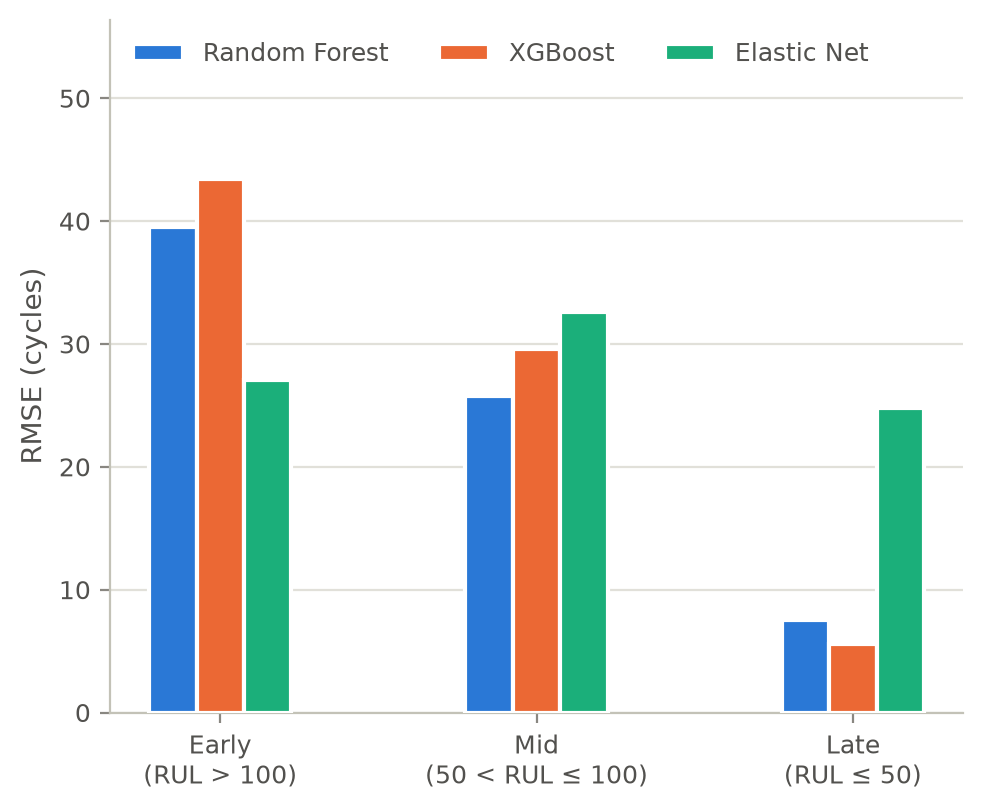
\includegraphics[width=0.92\columnwidth]{../../results/figures/fd001_test_stage_rmse.png}
\caption{Test RMSE by degradation stage of the true RUL for the engineered
models.}
\label{fig:stage_rmse}
\end{figure}

The early-stage errors are mostly overestimates. An engine whose sensors still
look healthy receives a long predicted life, typical of training engines that
lived 128 to 362 cycles, yet no test engine had more than 145 cycles left at its
last observed cycle. The engineered Random Forest overestimates 9 engines by more
than 50 cycles. Tree SHAP attributes far more of each engineered prediction to
\texttt{cycle} than to any sensor feature (Section~\ref{sec:models}), so for
young engines the models fall back on an age-based estimate and overestimate
their remaining life. Capping the training target roughly halves this error: the
engineered Random Forest's early-stage RMSE falls from 39.49 to 20.05 cycles,
still scored against the uncapped test RUL (Section~\ref{sec:capped}).

\begin{figure*}[!t]
\centering
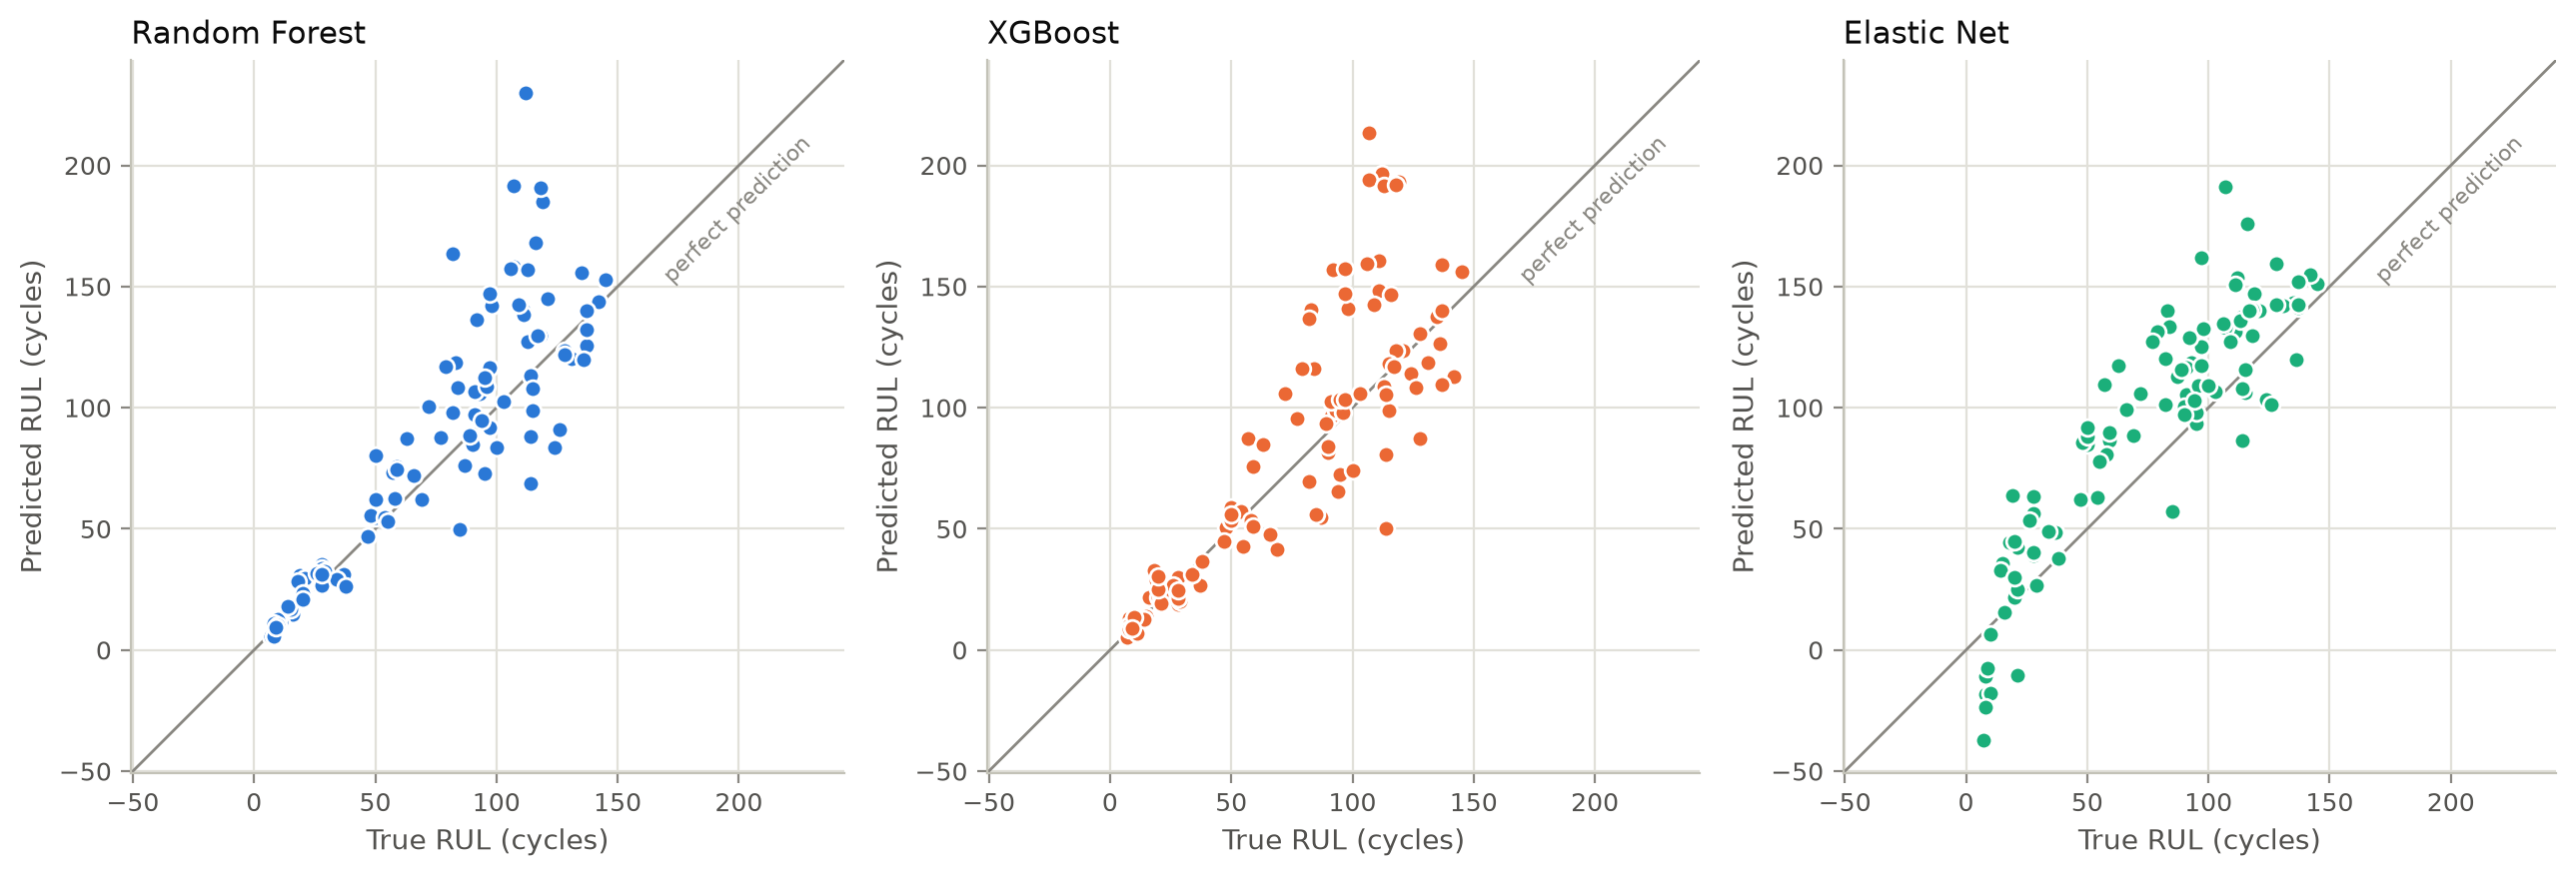
\includegraphics[width=\textwidth]{../../results/figures/fd001_test_pred_vs_true.png}
\caption{Predicted against true RUL at the last cycle of each test engine for the
engineered models. Points above the diagonal predict more life than the engine
had. The panels share one scale so that the Elastic Net's negative predictions
remain visible.}
\label{fig:pred_vs_true}
\end{figure*}

\subsection{Per-Engine Predictions}
Fig.~\ref{fig:pred_vs_true} shows the same pattern engine by engine: the
predictions are tight below about 50 cycles of true RUL and spread widely above
about 80. The Elastic Net predicts negative RUL for 7 test engines, since its
output is not bounded; the predictions are reported without clipping.
Fig.~\ref{fig:trajectories} follows the engineered Random Forest over the whole
recorded history of the four test engines observed longest, chosen by history
length rather than by error. These engines started with 270 to 330 cycles of
life, more than most training engines had, and early in each record the
prediction stays far below the true RUL. The gap narrows as degradation becomes
visible: at the last cycle, engines 49 and 62 are predicted within one cycle,
while engines 91 and 93 remain underestimated by 12 and 35 cycles, an early and
therefore safe error.

\begin{figure*}[!t]
\centering
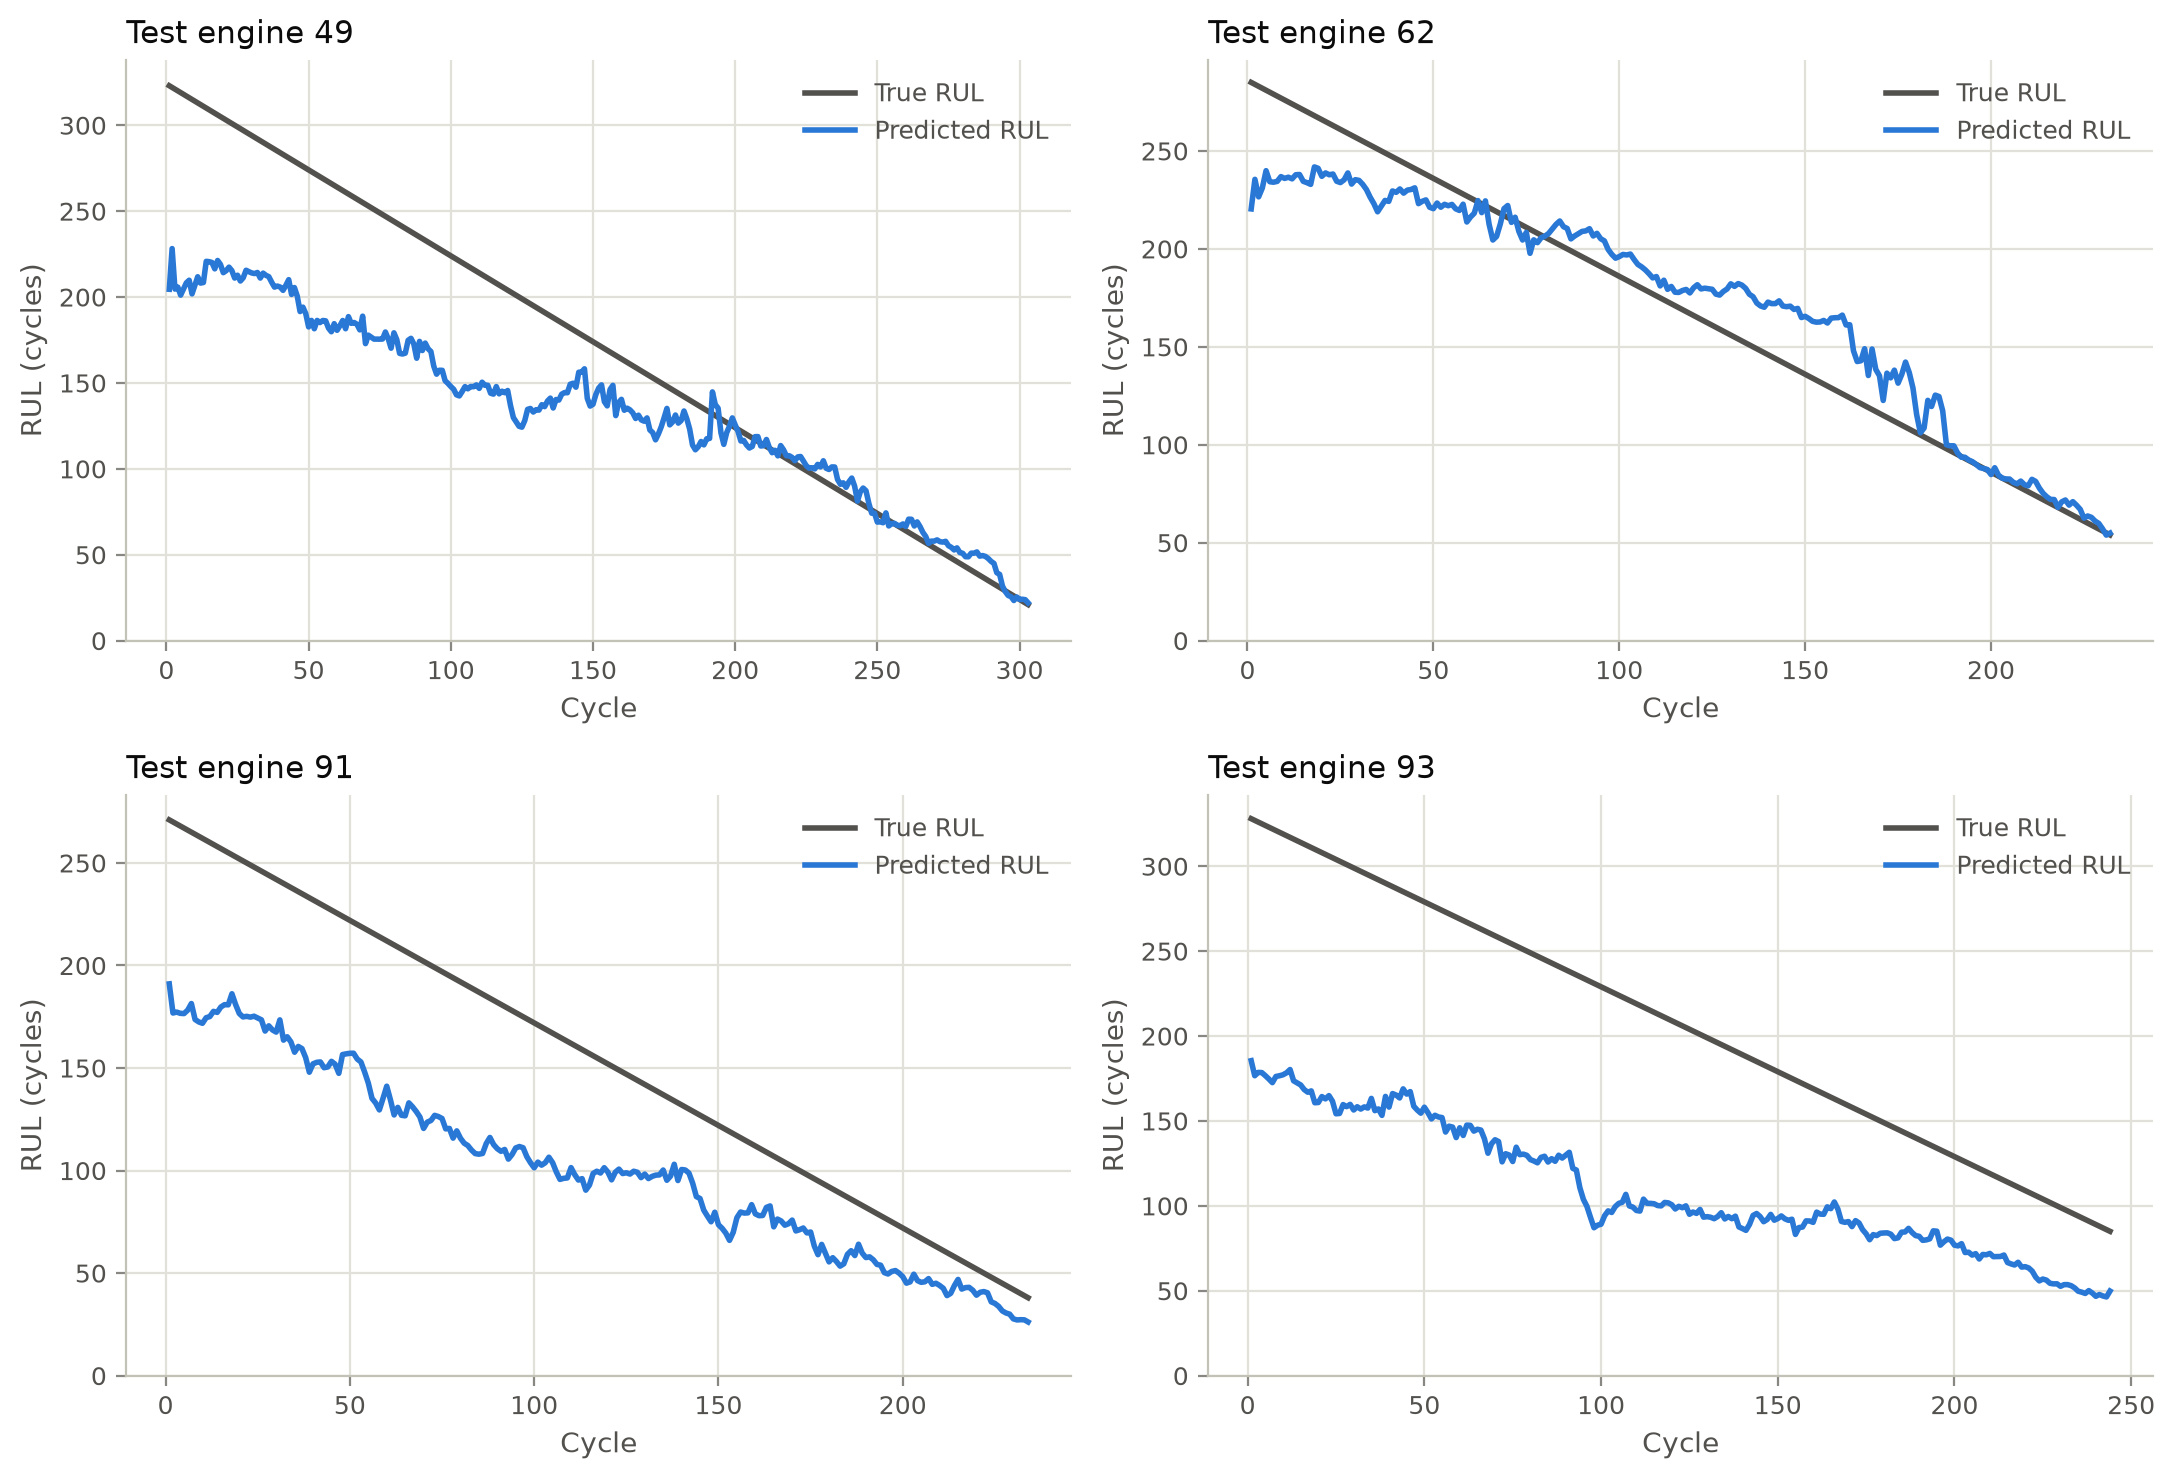
\includegraphics[width=0.78\textwidth]{../../results/figures/fd001_test_trajectories.png}
\caption{Engineered Random Forest predictions over the recorded cycles of the four
test engines with the longest histories (49, 62, 91 and 93), against the true
RUL.}
\label{fig:trajectories}
\end{figure*}

\subsection{Sensitivity of the NASA Score}
Because the NASA score is an exponential sum over engines, single engines
dominate it. Test engine~1 was observed for only 31 cycles and had 112 left; the
engineered Random Forest predicts 230. That one overestimate of 118 cycles
contributes 133{,}652 of the model's 145{,}410, or 92\%, while the other 99
engines add 11{,}758. XGBoost's largest single penalty is 68\% of its score. The
NASA ranking in Table~\ref{tab:test_results} is therefore driven by a handful of
young engines, which is why we read it together with RMSE, MAE and the stage
errors.

\subsection{Capped-Target Check}
\label{sec:capped}
To test whether the uncapped target explains the early-stage errors, Random
Forest was retrained with the training RUL capped at 125 cycles, using the same
grid, folds and seed, and scored against the true, uncapped test RUL
(Table~\ref{tab:capped}). Capping lowers the RMSE of both feature sets and
reverses their order: engineered features now reach 16.21 against 18.66 for raw
inputs, with an early-stage RMSE of 20.05 against 23.12 and a late-stage RMSE of
7.39 against 13.44. The comparison between feature sets therefore depends on how
RUL is defined. This is a single-model check with a cap taken from the
literature, not chosen on the test set; the full ablation over all models, with
the cap justified from training data, belongs to Phase~2.

\begin{table}[!t]
\centering
\caption{Random Forest test RMSE with the uncapped and the capped (125 cycles)
training target, scored against the true, uncapped test RUL.}
\label{tab:capped}
\begin{tabular}{lrr}
\hline
Training target & Engineered & Raw \\
\hline
Uncapped (primary)      & 27.55 & 26.15 \\
Capped at 125 (ablation) & 16.21 & 18.66 \\
\hline
\end{tabular}
\end{table}

% Conclusion and Phase 2 outlook (issue #7).

\section{Conclusion}
\label{sec:conclusion}

Phase~1 established a leakage-controlled protocol and feature-based baselines for
RUL prediction on C-MAPSS FD001. With 155 causal engineered features, the Random
Forest predicts the RUL of the 100 official test engines with an RMSE of 27.55
cycles and an MAE of 17.67, the lowest MAE of the six models; all six lie within
five RMSE cycles of each other. The overall numbers hide the main finding. Near
failure, where maintenance is decided, the engineered features roughly halve the
error of both tree models, to 7.52 and 5.62 cycles. Early in life, under the
uncapped target, they overestimate engines that still look healthy, and a single
such engine accounts for 92\% of the Random Forest's NASA score. Capping the
training target at 125 cycles removes much of this error and reverses the
raw-versus-engineered comparison, so conclusions about feature engineering
depend on how RUL is defined.

These results have limits. Only FD001, with one operating condition and one fault
mode, was evaluated, so regime normalization has not yet been tested where it
matters. Each model was tuned over a small grid with three folds, the XGBoost
learning rate was not tuned, and cross-validation scores every training cycle
rather than last cycles like the test set. Differences between models come from
one test set of 100 engines without confidence intervals, and the capped-target
result covers only the Random Forest.

Phase~2 keeps the splits, metrics and last-cycle scoring fixed and replaces the
fixed rolling summaries with sequence models, an LSTM, a temporal CNN and a
Transformer encoder, trained on sensor windows built inside engine boundaries.
A hybrid model will fuse a sequence encoder with the engineered-feature branch,
targeting the gap identified in Section~\ref{sec:introduction}. Ablations will
cover the capped target with the cap chosen on training data, window length,
feature groups and regime normalization on FD002 and FD004, and validation will
add repeated seeds, bootstrap confidence intervals and paired per-engine tests
using the saved predictions. The bar to beat is the Phase~1 method's test RMSE of
27.55 cycles (26.15 with raw inputs) and its late-stage RMSE of 6 to 8 cycles.

% Author contributions (issue #7), taken from the repository's commit history.

\section*{Author Contributions}
All code, notebooks and report sections are in the project repository, where each
file's history shows its author.
\begin{itemize}
\item \textbf{Gokul VKS} (lead): data loading and RUL labels, evaluation metrics
  and plots, official test scoring and the results notebook; literature review,
  introduction, methodology, results and conclusion; report assembly and code
  review.
\item \textbf{Milind Bansal}: engine-grouped splits, the exploratory data
  analysis notebook, operating-regime normalization, and the raw-versus-engineered
  comparison pipeline with its SHAP analysis.
\item \textbf{Isha Tomar}: sensor selection, rolling degradation features, the
  exported feature matrices and the feature-engineering notebook, and the
  baseline model wrappers.
\item \textbf{Yashi Agrawal}: the dataset and EDA and the models and theory
  sections, the consolidated references, the Phase~1 presentation and the
  capped-target check.
\item \textbf{Mohammad Affan Anas}: the data download script and data
  documentation, the setup and reproduction guide, and the feature engineering
  section.
\end{itemize}


\bibliographystyle{IEEEtran}
\bibliography{refs}

\end{document}
